\documentclass[journal,12pt,twocolumn]{IEEEtran}
\usepackage{setspace}
\usepackage{gensymb}
\singlespacing
\usepackage[cmex10]{amsmath}

\usepackage{amsthm}

\usepackage{mathrsfs}
\usepackage{txfonts}
\usepackage{stfloats}
\usepackage{bm}
\usepackage{cite}
\usepackage{cases}
\usepackage{subfig}

\usepackage{longtable}
\usepackage{multirow}
\usepackage{algorithm}
\usepackage{algorithmic}
\usepackage{enumitem}
\usepackage{mathtools}
\usepackage{steinmetz}
\usepackage{tikz}
\usepackage{circuitikz}
\usepackage{verbatim}
\usepackage{tfrupee}
\usepackage[breaklinks=true]{hyperref}
\usepackage{graphicx}
\usepackage{tkz-euclide}

\usetikzlibrary{calc,math}
\usepackage{listings}
    \usepackage{color}                                            %%
    \usepackage{array}                                            %%
    \usepackage{longtable}                                        %%
    \usepackage{calc}                                             %%
    \usepackage{multirow}                                         %%
    \usepackage{hhline}                                           %%
    \usepackage{ifthen}                                           %%
    \usepackage{lscape}     
\usepackage{multicol}
\usepackage{chngcntr}

\DeclareMathOperator*{\Res}{Res}

\renewcommand\thesection{\arabic{section}}
\renewcommand\thesubsection{\thesection.\arabic{subsection}}
\renewcommand\thesubsubsection{\thesubsection.\arabic{subsubsection}}

\renewcommand\thesectiondis{\arabic{section}}
\renewcommand\thesubsectiondis{\thesectiondis.\arabic{subsection}}
\renewcommand\thesubsubsectiondis{\thesubsectiondis.\arabic{subsubsection}}


\hyphenation{op-tical net-works semi-conduc-tor}
\def\inputGnumericTable{}                                 %%

\lstset{
%language=C,
frame=single, 
breaklines=true,
columns=fullflexible
}
\begin{document}


\newtheorem{theorem}{Theorem}[section]
\newtheorem{problem}{Problem}
\newtheorem{proposition}{Proposition}[section]
\newtheorem{lemma}{Lemma}[section]
\newtheorem{corollary}[theorem]{Corollary}
\newtheorem{example}{Example}[section]
\newtheorem{definition}[problem]{Definition}

\newcommand{\BEQA}{\begin{eqnarray}}
\newcommand{\EEQA}{\end{eqnarray}}
\newcommand{\define}{\stackrel{\triangle}{=}}
\bibliographystyle{IEEEtran}
\raggedbottom
\setlength{\parindent}{0pt}
\providecommand{\mbf}{\mathbf}
\providecommand{\pr}[1]{\ensuremath{\Pr\left(#1\right)}}
\providecommand{\qfunc}[1]{\ensuremath{Q\left(#1\right)}}
\providecommand{\sbrak}[1]{\ensuremath{{}\left[#1\right]}}
\providecommand{\lsbrak}[1]{\ensuremath{{}\left[#1\right.}}
\providecommand{\rsbrak}[1]{\ensuremath{{}\left.#1\right]}}
\providecommand{\brak}[1]{\ensuremath{\left(#1\right)}}
\providecommand{\lbrak}[1]{\ensuremath{\left(#1\right.}}
\providecommand{\rbrak}[1]{\ensuremath{\left.#1\right)}}
\providecommand{\cbrak}[1]{\ensuremath{\left\{#1\right\}}}
\providecommand{\lcbrak}[1]{\ensuremath{\left\{#1\right.}}
\providecommand{\rcbrak}[1]{\ensuremath{\left.#1\right\}}}
\theoremstyle{remark}
\newtheorem{rem}{Remark}
\newcommand{\sgn}{\mathop{\mathrm{sgn}}}
\providecommand{\abs}[1]{\left\vert#1\right\vert}
\providecommand{\res}[1]{\Res\displaylimits_{#1}} 
\providecommand{\norm}[1]{\left\lVert#1\right\rVert}
%\providecommand{\norm}[1]{\lVert#1\rVert}
\providecommand{\mtx}[1]{\mathbf{#1}}
\providecommand{\mean}[1]{E\left[ #1 \right]}
\providecommand{\fourier}{\overset{\mathcal{F}}{ \rightleftharpoons}}
%\providecommand{\hilbert}{\overset{\mathcal{H}}{ \rightleftharpoons}}
\providecommand{\system}{\overset{\mathcal{H}}{ \longleftrightarrow}}
	%\newcommand{\solution}[2]{\textbf{Solution:}{#1}}
\newcommand{\solution}{\noindent \textbf{Solution: }}
\newcommand{\cosec}{\,\text{cosec}\,}
\providecommand{\dec}[2]{\ensuremath{\overset{#1}{\underset{#2}{\gtrless}}}}
\newcommand{\myvec}[1]{\ensuremath{\begin{pmatrix}#1\end{pmatrix}}}
\newcommand{\mydet}[1]{\ensuremath{\begin{vmatrix}#1\end{vmatrix}}}
\numberwithin{equation}{subsection}
\makeatletter
\@addtoreset{figure}{problem}
\makeatother
\let\StandardTheFigure\thefigure
\let\vec\mathbf
\renewcommand{\thefigure}{\theproblem}
\def\putbox#1#2#3{\makebox[0in][l]{\makebox[#1][l]{}\raisebox{\baselineskip}[0in][0in]{\raisebox{#2}[0in][0in]{#3}}}}
     \def\rightbox#1{\makebox[0in][r]{#1}}
     \def\centbox#1{\makebox[0in]{#1}}
     \def\topbox#1{\raisebox{-\baselineskip}[0in][0in]{#1}}
     \def\midbox#1{\raisebox{-0.5\baselineskip}[0in][0in]{#1}}
\vspace{3cm}
\title{EE3025 FFT and IFFT Implementation}
\author{Ritwik Sahani - EE18BTECH11038}
\maketitle
\newpage
\renewcommand{\thefigure}{\theenumi}
\renewcommand{\thetable}{\theenumi}
\bigskip
Codes are available at 
\begin{lstlisting}
https://github.com/ritvix23/EE3025-IDP-DSP/tree/main/Assignment1_FFT/codes
\end{lstlisting}
To compile and run(on linux), navigate to the directory and execute- 
\begin{lstlisting}
gcc <filename>.c -o <filename> -lm && ./<filename>
\end{lstlisting}
\section{Problem}
Implement the Fast Fourier and Inverse Fast Fourier Transform algorithms in C to calculate DFT and Inverse DFT of a given sequence respectively. Verify using an example.

\section{Method}
The N-point Discrete Fourier Transform (DFT) for a given sequence $x[n]$ is defined by the formula - 

\begin{align}
X(k) = \sum_{n=0}^{N-1}x[n]W_{N}^{kn} \label{eq:eqn1}\\
W_N = e^\frac{-2\pi i}{N}
\end{align}
Upon collecting the odd indices and the even indices together, we get - 

\begin{align}
X(k) &= \sum_{r=0}^{\frac{N}{2}-1}x[2r]W_{N}^{(2r)k} + \sum_{r=0}^{\frac{N}{2}-1}x[2r+1]W_{N}^{(2r+1)k} \label{eq:eqn2}
\end{align}
Define     $e[r]=x[2r]$ and $o[r]=x[2r+1]$ , \\
Upon  substituting this in equation \ref{eq:eqn2}, we get
\begin{align}
    X(k) &= \sum_{r=0}^{\frac{N}{2}-1}e[r]W_{N/2}^{kr} + W_{N}^k\sum_{r=0}^{\frac{N}{2}-1}o[r]W_{N/2}^{kr}
    \label{eq:eq3}
\end{align}

At this point, we can exploit the following property of complex exponentials, along with peridocity, to get a recursive definition of $X(k)$ - 
\begin{align}
    W_\frac{N}{2} = W_{N}^{2}
\end{align}
which gives - 

\begin{align}
    X(k) &= E(k) + W_{N}^k O(k) \text{   } \forall \text{ k in } [0, ..., N/2] \label{eq:eqn4}\\
    X(k) &= E(k) - W_{N}^k O(k) \text{   } \forall \text{ k in } [N/2+1, ..., N]\label{eq:eqn5}
\end{align}
If we assume the input length to be a power of two, a recursive algorithm can be designed from equations \ref{eq:eqn4} and \ref{eq:eqn5}  as follows - 


\begin{algorithm}
\caption{FFT(x)}
\begin{algorithmic} 
% \STATE $n = length (x)$ such that $n = 2^k$
\IF{$N > 1$}
\STATE $E =FFT$ (x[0],x[2]...,x[N-2])
\STATE  $O =FFT$ (x[1],x[3]...,x[N-1])
\FOR{$k \longleftarrow 0 $ to $\frac{N}{2}-1$ }
\STATE $x[k]$= $E[k]$ + $e^{-2\pi jk/N}$ $O[k]$
\STATE $x[k+ \frac{N}{2}]$= $E[k]$ - $e^{-2\pi jk/N}$ $O[k]$
\ENDFOR
\ENDIF
\STATE return x

\end{algorithmic}
\end{algorithm}
The following C code first generates the DFT of the input and then performs IDFT on the resulting sequence. The given input is - {\brak{0, 9, 1, 1, 2, 0, 0, 1}}. The output of both the operations are printed and stored in a DAT file.
\begin{lstlisting}
https://github.com/ritvix23/EE3025-IDP-DSP/blob/main/Assignment1_FFT/codes/transform.c
\end{lstlisting}
The following python code reads the data from the DAT file and plots its frequency spectrum.
\begin{lstlisting}
https://github.com/ritvix23/EE3025-IDP-DSP/blob/main/Assignment1_FFT/codes/plot.py
\end{lstlisting}
The spectrum of the DFT from the inbuilt routine in Python Numpy is plotted for verification using - 
\begin{lstlisting}
https://github.com/ritvix23/EE3025-IDP-DSP/blob/main/Assignment1_FFT/codes/verify.py
\end{lstlisting}
\begin{figure}
    \centering
    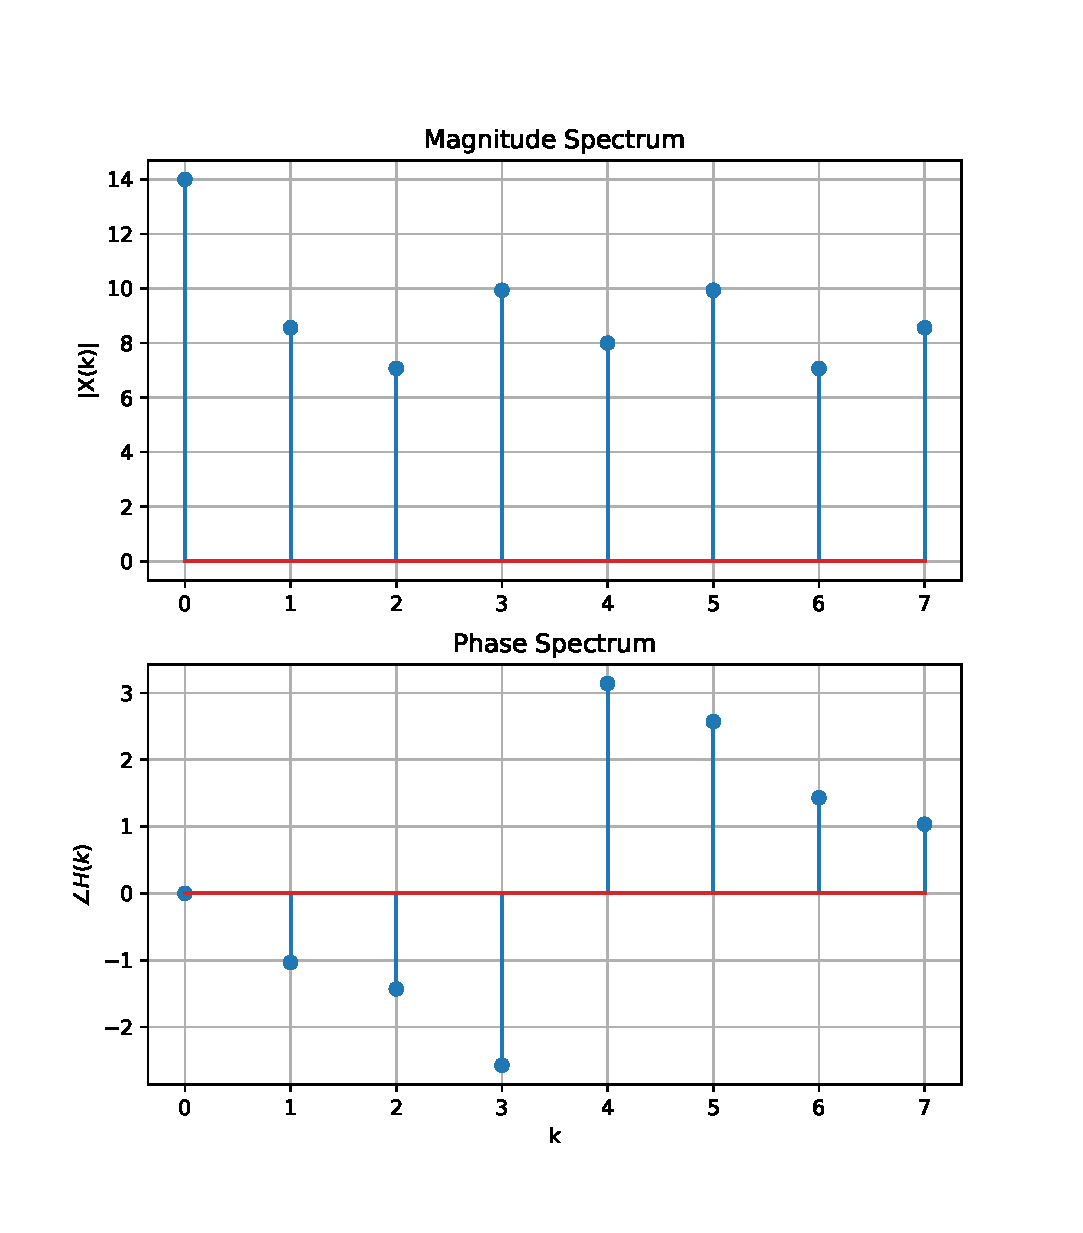
\includegraphics[width=\columnwidth]{./figs/dftown.eps}
    \caption{From own routine}
    \label{fig:dftown}
\end{figure}
\begin{figure}
    \centering
    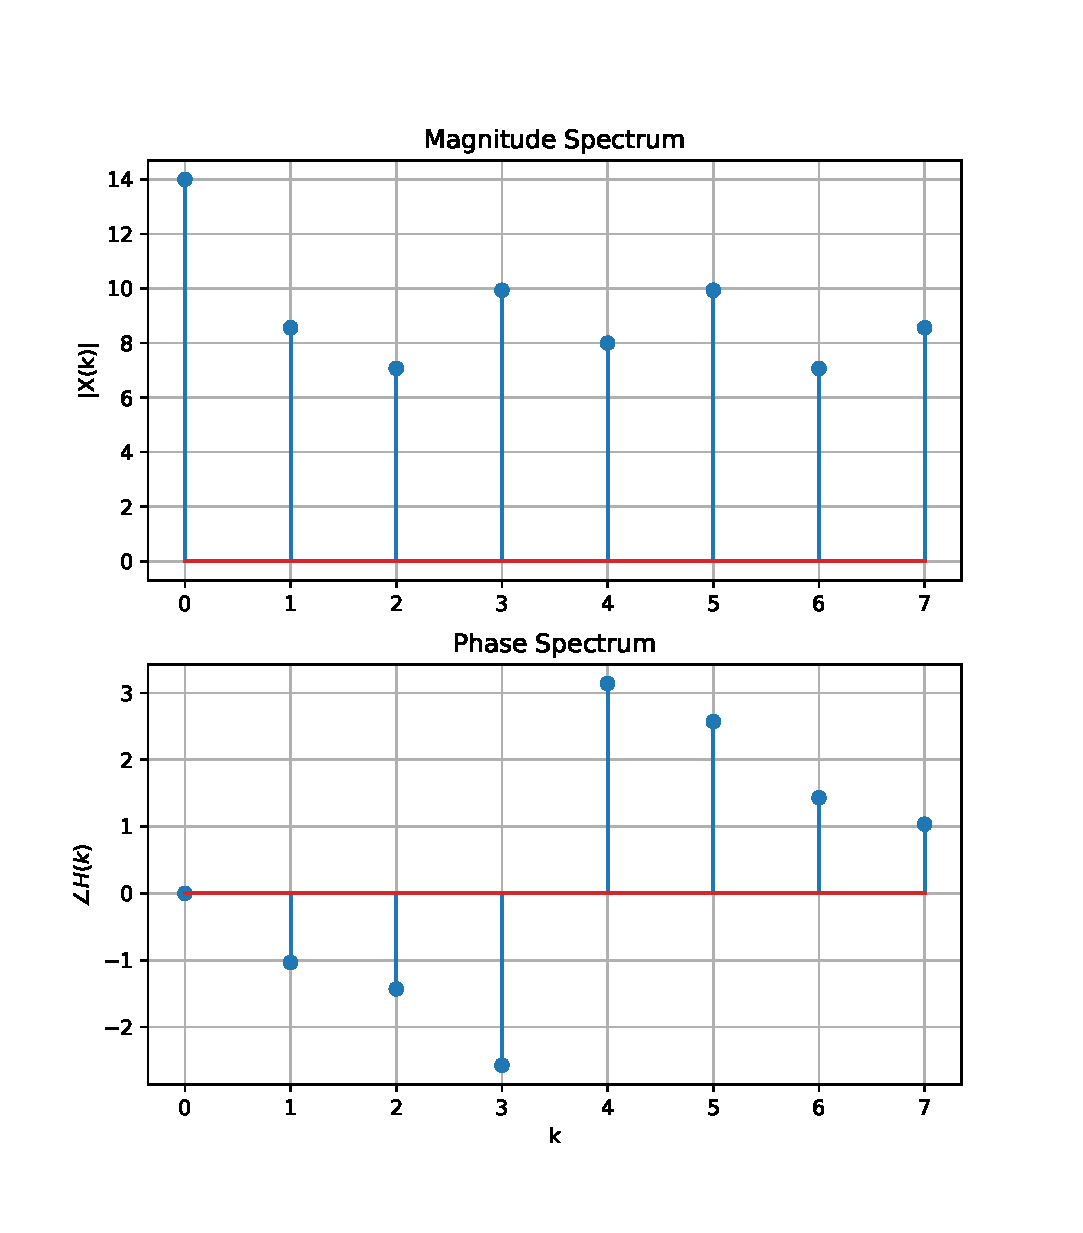
\includegraphics[width=\columnwidth]{./figs/dftnumpy.eps}
    \caption{From builtin routine}
    \label{fig:dftnumpy}
\end{figure}

\end{document}